% =====================================================================
% MDPI *Entropy* submission --- single-file source.
%
% REQUIRES the Entropy LaTeX template support files, which are NOT in this repo.
% Download "LaTeX template" from https://www.mdpi.com/journal/entropy/instructions
% and place into doc/:  Definitions/mdpi.cls, the Definitions/ logo files, and
% mdpi.bst (the bibliography style).  This file will NOT compile until they exist.
%
% Build: pdflatex -> bibtex -> pdflatex -> pdflatex  (uses article.bib).
% =====================================================================
\documentclass[entropy,article,submit,oneauthor,pdftex]{Definitions/mdpi}

% Packages the MDPI class does not already load (it provides amsmath, amsthm,
% amssymb, enumitem, tikz, graphicx, hyperref, natbib, array, booktabs, caption).
% Note: do NOT load `cite' --- the MDPI class uses natbib and the two conflict.
\usepackage{annotate-equations}
\usetikzlibrary{arrows}
\usepackage{pgfplots}
\pgfplotsset{compat=1.16}
\usetikzlibrary{arrows.meta,positioning}
\usepackage{euscript}
\usepackage{wasysym} % upright integration symbols (\varint)
\usepackage{delarray}

% The MDPI class already defines the (capitalised) Proposition environment; the body
% uses \begin{Proposition}. Do NOT \newtheorem{proposition} --- it clashes with the
% class's `proposition' counter.

\newcommand\drawbits[1]{%
    \tikz[x=1.5ex,y=1.5ex,sharp corners,every path/.style={draw=black,semithick}]{
        \foreach \y [count=\i] in {#1} {
            \expandafter\ifx\y0
            \draw (\i,0) rectangle (\i+1,1);
            \else
                            \draw (\i,0) rectangle (\i+1,1);
                            \filldraw[fill=black] (\i+0.2,0.2) rectangle (\i*1+0.8,0.8);
            \fi
        }
    }
}

% --- MDPI front matter ---
\firstpage{1}
\makeatletter
\setcounter{page}{\@firstpage}
\makeatother
\pubvolume{1}
\issuenum{1}
\articlenumber{0}
\pubyear{2026}
\copyrightyear{2026}
\datereceived{}
\dateaccepted{}
\datepublished{}

\Title{Combinadic Compression: An Order-0 Enumerative Byte-Stream Codec with Size-Preserving Encryption}
\Author{Anthony J.~Rasmussen\,\href{https://orcid.org/0009-0003-3924-319X}{\orcidicon}}
\AuthorNames{Anthony J. Rasmussen}
\address{%
Shack C Technologies, Australia; anthony@shackc.tech}
\corres{Correspondence: anthony@shackc.tech}

\abstract{Order-$0$ enumerative coding represents a fixed-length block not as a
self-delimiting bitstream but as a short tuple of integer fields over known finite ranges:
each byte value's positions form a bitset which, after a length-reduction step, becomes its
colexicographic rank, leaving per-symbol counts and ranks. We take this
\emph{representation}, not a particular codec, as the object of study, and show that this one
structural fact---finite-range integer fields---affords properties that a self-delimiting
bitstream does not. It is order-$0$-optimal, reaching the entropy bound up to an $O(A\log N)$
per-block overhead; against the Huffman, range, and ANS coders at matched block sizes it is
the most compact of the \emph{block-resetting} order-$0$ coders on narrow alphabets, though a
globally-modelled coder is more compact at small blocks. Because every field is an integer
over a known range, the representation also yields an exact compressed size known before
encoding, independent random access, and an in-place size-preserving cipher (addition modulo
each range) reducing to a standard keystream. Leaving the counts in clear exposes only a
block's count spectrum---an adjustable leakage equal to that spectrum's entropy, small on
the homogeneous streams it best suits.
Slower than streaming coders at equal ratio, it is offered not as a general-purpose
compressor but as a structurally transparent point in the design space, suited to record
stores and constrained-alphabet data.}

\keyword{lossless compression; enumerative coding; combinatorial number system;
binomial coefficient; colexicographic ordering; size-preserving encryption; joint
compression and encryption}

\begin{document}

\section{Introduction}\label{sec:introduction}
All digital data---photographs, documents, database tables---is ultimately a
stream of bytes, and there is a great deal of it. Despite cheap, abundant storage
and bandwidth, it remains worthwhile to compress data before writing it to disk
or sending it over a network, and there is no shortage of utilities that do so:
\texttt{gzip}, \texttt{bzip2}, \texttt{xz}, \texttt{zstd}, and many others.

Broadly, modern lossless compressors combine two ingredients. A \emph{model}
predicts or removes redundancy---dictionary and match-based methods such as
LZ77/LZ78~\cite{ziv1977,ziv1978}, the Burrows--Wheeler transform~\cite{burrows1994},
and adaptive context models~\cite{cleary1984}---and an
\emph{entropy coder} represents the residual symbols in close to their
information-theoretic minimum. The entropy stage is itself a mature field:
Huffman coding~\cite{huffman1952}, arithmetic coding~\cite{witten1987arithmetic},
range coding~\cite{martin1979}, and
the more recent asymmetric numeral systems~\cite{duda2013ans} all approach the
order-$0$ entropy of their input, differing mainly in speed and in how the coding
state is carried.

This article concerns a less common member of the entropy-coding family:
\emph{enumerative coding}~\cite{cover1973enumerative}. The idea is exact rather
than statistical---one assigns every admissible sequence a unique index in the
lexicographic (or, here, colexicographic) ordering of the set it belongs to, and
transmits that index in place of the sequence. For the set of binary sequences of
a fixed weight, the index is a sum of binomial coefficients, and both the index
and its inverse are computed in closed form~\cite{lynch1966,schalkwijk1972}.
Enumerative coding meets the order-$0$ entropy bound by construction and requires
no probability model, but it has seen limited use as a general byte-stream
compressor, in part because the indices are large integers whose arithmetic is
slower than a streaming coder's.

Our object of study is the \emph{representation} this coding induces, more than any
particular codec. A stream is divided into fixed-length blocks; within each block the
positions of every byte value form disjoint bitsets, which---after a length-reduction step
that re-expresses each bitset in the coordinate space left by those already encoded---are
replaced by their colexicographic ranks. A block is thereby a short tuple of integer
fields---the per-symbol counts and these ranks---each over a known finite range. It is this
one structural fact---finite-range integer fields rather than a self-delimiting
bitstream---that affords a family of properties a streaming entropy coder cannot, and which
we realise as a codec, characterise, and analyse. The contributions of this paper are:

\begin{itemize}[label=$\bullet$]
  \item a realisation of this representation as a byte-stream codec---the per-symbol ranking
        is classical (Cover; Schalkwijk), applied in its multinomial form block-wise over the
        full byte alphabet, the most-frequent value recovered by elimination
        (Sections~\ref{sec:mathematical-preliminaries}--\ref{sec:decompression-algorithm});
  \item a characterisation of the representation against mainstream coders---an
        allocation-light, block-parallel implementation (Section~\ref{sec:implementation})
        whose compressed size and throughput we measure against the entropy coders of a
        modern compressor on the \texttt{enwik9} benchmark, finding it order-$0$-optimal and,
        on narrow-alphabet inputs, the most compact of these \emph{block-resetting} coders at
        a matched block size, while on wide-alphabet data its per-block housekeeping overtakes
        the gain (Section~\ref{sec:computational-experiments});
  \item the setting these properties suit---the \emph{homogeneous record store}, where small,
        externally fixed blocks are the unit of storage and access. There the representation
        supplies as a single package what a streaming entropy coder cannot: order-$0$-compact
        ratios that lead the \emph{block-resetting} order-$0$ coders on constrained alphabets,
        independent random access, an exact compressed size known before encoding, and the
        cipher below---with embedded pipelines, packet and record stores, and short-read
        genomics the natural settings (Section~\ref{sec:applications}); and
  \item a size-preserving cipher the representation admits directly
        (Section~\ref{sec:encryption}): because each field is an integer over a known range,
        every field is encrypted in place at no size cost. Full encryption matches per-record
        AES-CTR on size, access, and leakage; leaving the counts in clear gives a tunable,
        key-less computability whose disclosure we characterise information-theoretically as
        $I(\text{content};\text{leak})=H(S)$, the entropy of the count spectrum---small, with
        its query value, on homogeneous data. We present this as a structural property of the
        representation, with stated assumptions and leakage, not as a deployed feature.
\end{itemize}

The remainder of the article is organised as follows.
Section~\ref{sec:related-work} situates the method among related compression and
joint-encryption schemes. Section~\ref{sec:mathematical-preliminaries} fixes
notation and the ranking machinery; Sections~\ref{sec:compression-algorithm}
and~\ref{sec:decompression-algorithm} present the encoder and decoder;
Section~\ref{sec:encryption} develops the size-preserving cipher and its security;
Section~\ref{sec:implementation} describes the implementation;
Section~\ref{sec:computational-experiments} reports experiments;
Section~\ref{sec:applications} discusses applications;
Section~\ref{sec:discussion} weighs limitations and positioning; and
Section~\ref{sec:conclusions} concludes.
\section{Related work}\label{sec:related-work}
\subsection{Enumerative coding}
The technique on which this work rests is enumerative source
coding~\cite{cover1973enumerative}: a sequence is represented by its index in the
ordered enumeration of the set $S$ of admissible sequences, so that storing the index
achieves compression of $(\log_2|S|)/n$ bits per symbol. Cover gives closed-form
indices for two cases of particular interest, sequences of a fixed weight and
sequences with a prescribed empirical Markov property, and an efficient inverse.
The fixed-weight case had been treated earlier by
Lynch~\cite{lynch1966} and Schalkwijk~\cite{schalkwijk1972}---hence
``Lynch--Davisson'' or combinatorial coding---and was later subsumed by
Rissanen's arithmetic framework~\cite{rissanen1976}. Our per-symbol step is
exactly the enumerative coding of a constant-weight bitset, and the full block
decomposition is the classical multinomial enumeration of a multiset permutation;
the present contribution is therefore not the enumerative kernel but its realisation
as a practical byte-stream codec---the block-parallel implementation, the systematic
comparison against mainstream coders, and the joint-encryption variant.

Borysenko and co-workers have independently developed a closely related line
of work under the name \emph{binomial
compression}~\cite{borysenko2021bns,borysenko2022adaptive,kulyk2025speedup}.
Their scheme encodes fixed-length blocks of binary sequences as binomial
numbers---the colexicographic rank of a constant-weight bitset---and an
adaptive variant adds an early-exit rule that bypasses the ranking step for
blocks whose unit count falls outside an efficient compression range,
recovering throughput at the cost of a ratio penalty of up to three to five
percent~\cite{kulyk2025speedup}. The present work differs in three
respects. First, where their scheme treats only binary (constant-weight)
sequences, ours codes the full byte alphabet via the multinomial factorisation
of the rank---a product of binomial coefficients over all distinct symbol values. This distinction is consequential for
compression quality: a bit-stream coder cannot capture correlations between
bit positions within a byte, so for typical byte-oriented data such as text
the bit-level entropy is near $1$ bit per bit and the binary scheme achieves
almost no compression, whereas the byte-stream formulation attains the
(substantially lower) order-$0$ byte entropy at every block size.
Second, it provides a systematic experimental
comparison against mainstream streaming coders---Huffman, range, and
ANS---at matched block sizes on standard corpora. Third, it derives a
joint compression-and-encryption construction from the finite-range property
of the rank (Section~\ref{sec:encryption}). The binomial-number-system line has
itself gestured at protecting information from unauthorised access through the
structure of the encoding, but that protection rests on the obscurity of the number
system rather than a key; our construction is instead a keyed, size-preserving
cipher whose confidentiality reduces to that of a standard keystream, with stated
assumptions and leakage.
\subsection{Statistical entropy coders}
The practical alternatives to enumerative coding at the same (order-$0$) bound are
the streaming statistical coders. Huffman coding is optimal among prefix codes
but integral-length; arithmetic coding~\cite{witten1987arithmetic} and range
coding remove the integrality penalty by maintaining a fractional interval; and
asymmetric numeral systems~\cite{duda2013ans} attain arithmetic-coding ratios at
table-driven speeds and now underlie several mainstream compressors. Like
enumerative coding, arithmetic coding maps a message to a number; the essential
differences are that it is adaptive and renormalised, and that our index is an
exact rank over a finite combinatorial set rather than a point in a real
interval. As our experiments confirm
(Section~\ref{sec:computational-experiments}), these coders reach the same
compressed size as our method while running substantially faster, so our
motivation lies in the structural properties of the combinatorial representation
rather than in throughput.

\subsection{Succinct combinatorial representations}
The same combinatorial index that we use to compress a bitset is the basis of
succinct data structures. The indexable-dictionary scheme of Raman, Raman and
Rao~\cite{raman2002succinct} encodes a bitvector as a (class, offset) pair---the
class being its weight and the offset its enumerative index---and supports
constant-time rank and select queries on the compressed form. Our encoder
produces the same kind of object per byte value, which makes the construction a
natural building block for compressed-but-queryable representations such as
bitmap indexes and inverted-index posting lists.

\subsection{Joint compression and encryption}
Because the entropy stage of a compressor maps data onto a near-uniform code, it
is a natural place to introduce a cipher. Randomized arithmetic
coding~\cite{grangetto2006rac} encrypts by making the coder's interval
assignment depend on a secret key, achieving compression and encryption together
at negligible cost in efficiency; related schemes randomise binary arithmetic
coders or Huffman trees. Our variant follows the same principle but exploits a
property specific to enumerative coding: every field of a block is an integer
over a known finite range, so it can be encrypted by a modular cipher that is
exactly size-preserving (Section~\ref{sec:encryption}), rather than by
randomising the internal state of a streaming coder.

\emph{Format-preserving encryption} (FPE) is the direct point of comparison. It
encrypts a value so that the ciphertext inhabits the same domain---an integer in
$[0,M)$ to an integer in $[0,M)$, a card number to a card number. The standard
constructions are pseudorandom permutations over the domain, built as Feistel
networks: the FFX mode of Bellare, Rogaway and Spies~\cite{bellare2010ffx}, standardised
by NIST as FF1 and FF3 in SP~800-38G~\cite{dworkin2016fpe}, descends from the problem of
ciphers over arbitrary finite domains~\cite{black2002arbitrary}. That line has proved
delicate: FF3 fell to Durak and Vaudenay~\cite{durak2017ff3}, its repaired variant
FF3-1 to Beyne~\cite{beyne2021ff31}, and a 2025 draft revision of the standard removes
FF3 altogether, leaving FF1. Our cipher achieves the same domain preservation---each
field's ciphertext stays in its own range $[0,M)$, so the encrypted block is exactly
the size of the plaintext---and we call it \emph{size-preserving} encryption, reserving
``format-preserving'' for the permutation-based family above. It is a different
primitive: not a deterministic pseudorandom permutation but a randomised additive stream
cipher over $\mathbb{Z}_M$ (a one-time pad keyed by a nonce-addressed keystream), whose
confidentiality reduces to that of a standard stream cipher rather than to a bespoke
Feistel network. The trade is
deliberate. We give up the deterministic, equality-preserving behaviour that
permutation-based FPE provides, and that some tokenisation settings rely on, in exchange
for semantic security and a reduction to a well-understood primitive that has not
needed the repeated repair the FFX line has; the cost is that an additive cipher is
malleable and so wants per-block authentication, which we treat as deferred hardening
(Section~\ref{sec:encryption}).

We develop the full
construction---its tunable leakage--queryability dial and a security analysis---in
Section~\ref{sec:encryption}.

\section{Mathematical preliminaries}\label{sec:mathematical-preliminaries}
Let a bitset contain $N$ bits and have a population count of $k$.
Bitset $b$ is one of many possible bitsets associated with the tuple $(N,k)$, or $b\in{B_{N,k}}=\{b_0, b_1, \dots\}$.
The cardinality of $B_{N,k}$ is given by the usual binomial coefficient
\begin{equation}
|B_{N,k}|=\binom{N}{k}=\frac{N!}{k!(N-k)!}.
\end{equation}

Using colexicographic ordering, there is a ranking function to obtain the index value of each $b$ in $B_{N,k}$:
\begin{equation}
r(b)=\sum^{k}_{i=1}\binom{p(b,i)}{i}\label{eq:rank}
\end{equation}
where $p(b,i)\in{[0,N-1]}$ gives the $i$th \emph{on} position within $b$. This rank is the
\emph{combinadic} of $b$---its representation in the combinatorial number system, which
gives this paper its title.

Clearly, for a known value of $N$, bitset compression can be achieved with a ranking function whenever
\vspace{1.5\baselineskip}
\begin{equation}
    \eqnmark[black]{node1}{\lceil\log_2(N+1)\rceil}
    \tikzmarknode{node2}{+}
    \eqnmark[black]{node3}{\lceil\log_2\binom{N}{k}\rceil}
    \tikzmarknode{node4}{<N}.
    \annotate[yshift=-0.35em]{below,left}{node1}{cost of storing $k$}
    \annotate[yshift=0.5em]{above,right}{node3}{cost of storing $r$}
\end{equation}
\vspace{1.5\baselineskip}

We can recover the ordered set $\{p(b,k),\dots,p(b,1)\}$ from $r(b)$ and $k$ by unranking as follows
\begin{equation}
p(b,i)=\max\Big\{\,j:\binom{j}{i}\leqslant r(b)-\sum^{k}_{\ell=i+1}\binom{p(b,\ell)}{\ell}\Big\}.
\end{equation}

\section{Compression algorithm}\label{sec:compression-algorithm}
For a large file, it is tempting to consider a single compression step as prescribed in eq.~\eqref{eq:rank}.
This is rarely practical, however, as it leads to the expensive computation of binomial coefficients with very large arguments.
Instead, it is prudent to consider compressing smaller, fixed-width blocks.

The next temptation is to apply compression to all raw bits in every block.
While this is certainly less expensive than single-step compression, more efficiencies become available by analysing
the bytes within each block.

Consider a block containing 20 bytes in which only five byte values occur: \texttt{dbcbc\allowbreak eaeec\allowbreak bacdc\allowbreak ecbeb}. We map each byte value to a bitset marking the positions it occupies within the block---the per-value bitsets in the second stage of Figure~\ref{fig:pipeline}.

\begin{figure}[htbp]
\centering
\begin{tikzpicture}[
  font=\small,
  stage/.style={draw=black!55, rounded corners=2pt, fill=black!3,
                inner sep=6pt, align=center},
  flow/.style={-{Latex[length=2.4mm]}, black!65, thick},
  oplabel/.style={font=\footnotesize\itshape, fill=white, inner sep=1.5pt},
]

\node[stage] (blk) {%
  \textbf{Block} \;--\; $N=20$ bytes, alphabet $\{a,b,c,d,e\}$\\[3pt]
  \ttfamily d\,b\,c\,b\,c\,e\,a\,e\,e\,c\,b\,a\,c\,d\,c\,e\,c\,b\,e\,b
};

\node[stage, below=9mm of blk] (bits) {%
  \textbf{Per-value bitsets} \;--\; the positions each byte value occupies\\[4pt]
  \begin{tabular}{r@{\;\;}l}
   $a$ & \drawbits{0,0,0,0,0,0,1,0,0,0,0,1,0,0,0,0,0,0,0,0}\\
   $b$ & \drawbits{0,1,0,1,0,0,0,0,0,0,1,0,0,0,0,0,0,1,0,1}\\
   $c$ & \drawbits{0,0,1,0,1,0,0,0,0,1,0,0,1,0,1,0,1,0,0,0}\\
   $d$ & \drawbits{1,0,0,0,0,0,0,0,0,0,0,0,0,1,0,0,0,0,0,0}\\
   $e$ & \drawbits{0,0,0,0,0,1,0,1,1,0,0,0,0,0,0,1,0,0,1,0}\\
  \end{tabular}
};

\node[stage, below=9mm of bits] (red) {%
  \textbf{Reduce, most-frequent value last}\\ universe shrinks
  $20\!\to\!18\!\to\!13\!\to\!11\!\to\!6$\\[4pt]
  \begin{tabular}{r@{\;\;}l@{\qquad}l}
   $a$  & \drawbits{0,0,0,0,0,0,1,0,0,0,0,1,0,0,0,0,0,0,0,0} & \footnotesize $k{=}2$, ranked over $20$\\
   $b'$ & \drawbits{0,1,0,1,0,0,0,0,0,1,0,0,0,0,0,1,0,1}     & \footnotesize $k{=}5$, ranked over $18$\\
   $d'$ & \drawbits{1,0,0,0,0,0,0,0,1,0,0,0,0}               & \footnotesize $k{=}2$, ranked over $13$\\
   $e'$ & \drawbits{0,0,1,1,1,0,0,0,1,0,1}                   & \footnotesize $k{=}5$, ranked over $11$\\
   $c'$ & \drawbits{1,1,1,1,1,1}                             & \footnotesize $k{=}6$, inferred (not ranked)\\
  \end{tabular}
};

\node[stage, below=9mm of red] (pack) {%
  \textbf{Rank \& pack} \;--\; each reduced bitset becomes its\\
  colexicographic rank, an integer over a known range\\[5pt]
  % the packed block, bit for bit (filled square = 1): header row, then the per-value pairs
  \begin{tikzpicture}[x=0.22cm, y=0.22cm, sharp corners,
     bx/.style={draw=black!55, line width=0.2pt}, alab/.style={font=\footnotesize, inner sep=1pt}]
   % row 1 -- header: cardinality, alphabet rank, MFV, count width
   \foreach \i/\c in {%
      0/violet!28,1/violet!28,2/violet!28,3/violet!28,4/violet!28,5/violet!28,6/violet!28,7/violet!28,8/violet!28,
      9/blue!14,10/blue!14,11/blue!14,12/blue!14,13/blue!14,14/blue!14,15/blue!14,16/blue!14,17/blue!14,
      18/blue!14,19/blue!14,20/blue!14,21/blue!14,22/blue!14,23/blue!14,24/blue!14,25/blue!14,26/blue!14,
      27/blue!14,28/blue!14,29/blue!14,30/blue!14,31/blue!14,32/blue!14,33/blue!14,34/blue!14,35/blue!14,
      36/blue!14,37/blue!14,38/blue!14,39/blue!14,40/blue!14,41/blue!14,42/blue!14,
      43/blue!30,44/blue!30,45/blue!30,46/blue!30,47/blue!30,48/blue!30,49/blue!30,50/blue!30,
      51/black!12,52/black!12,53/black!12,54/black!12,55/black!12}{%
      \fill[\c] (\i,0) rectangle (\i+1,1); \draw[bx] (\i,0) rectangle (\i+1,1);}
   \foreach \i in {6,8,16,19,20,21,22,24,25,27,28,29,31,32,33,38,40,42,44,45,49,50,54,55}{%
      \fill[black!80] (\i+0.22,0.22) rectangle (\i+0.78,0.78);}
   \node[anchor=west, font=\large] at (57,0.5) {$+$};
   % row 2 -- the (count, rank) pair for each remaining value
   \foreach \i/\c in {%
      0/orange!24,1/orange!24,2/orange!24,3/green!20,4/green!20,5/green!20,6/green!20,7/green!20,8/green!20,
      9/green!20,10/green!20,11/orange!24,12/orange!24,13/orange!24,14/green!20,15/green!20,16/green!20,
      17/green!20,18/green!20,19/green!20,20/green!20,21/green!20,22/green!20,23/green!20,24/green!20,
      25/green!20,26/green!20,27/green!20,28/orange!24,29/orange!24,30/orange!24,31/green!20,32/green!20,
      33/green!20,34/green!20,35/green!20,36/green!20,37/green!20,38/orange!24,39/orange!24,40/orange!24,
      41/green!20,42/green!20,43/green!20,44/green!20,45/green!20,46/green!20,47/green!20,48/green!20,
      49/green!20}{%
      \fill[\c] (\i,-4) rectangle (\i+1,-3); \draw[bx] (\i,-4) rectangle (\i+1,-3);}
   \foreach \i in {1,5,6,7,8,10,11,13,15,16,17,19,20,21,23,24,27,29,33,34,35,38,40,41,43,46,48,49}{%
      \fill[black!80] (\i+0.22,-3.78) rectangle (\i+0.78,-3.22);}
   \node[font=\footnotesize, anchor=west] at (51,-3.5) {($106$ bits)};
  \end{tikzpicture}\\[6pt]
  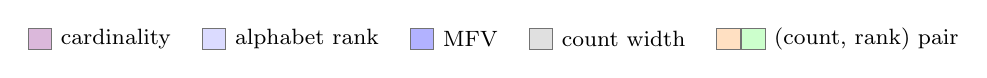
\begin{tikzpicture}[font=\footnotesize, sharp corners,
     sw/.style={draw=black!55, line width=0.3pt, minimum width=3mm, minimum height=2.6mm, inner sep=0pt},
     lbl/.style={inner sep=0pt}]
   \node[sw, fill=violet!28] (s1) {};
   \node[lbl, right=3pt of s1]  (l1) {cardinality};
   \node[sw, fill=blue!14, right=11pt of l1] (s2) {};
   \node[lbl, right=3pt of s2]  (l2) {alphabet rank};
   \node[sw, fill=blue!30, right=11pt of l2] (s3) {};
   \node[lbl, right=3pt of s3]  (l3) {MFV};
   \node[sw, fill=black!12, right=11pt of l3] (s4) {};
   \node[lbl, right=3pt of s4]  (l4) {count width};
   \node[sw, fill=orange!24, right=11pt of l4] (s5) {};
   \node[sw, fill=green!20, right=0pt of s5]  (s6) {};
   \node[lbl, right=3pt of s6]  (l5) {(count,~rank) pair};
  \end{tikzpicture}
};

\draw[flow] (blk)  -- (bits) node[oplabel,midway,right] {map};
\draw[flow] (bits) -- (red)  node[oplabel,midway,right] {reduce};
\draw[flow] (red)  -- (pack) node[oplabel,midway,right] {rank \& pack};
\end{tikzpicture}
\caption[The per-block pipeline on the running example.]{The per-block pipeline on the
running example, the $20$-byte block \texttt{dbcbceaeecbacdcecbeb} over $\{a,b,c,d,e\}$:
each byte value's positions form a bitset, reduced in most-frequent-last order and replaced
by its colexicographic rank. The final stage shows the \emph{actual} packed block bit for
bit (filled\,$=$\,\protect\drawbits{1}), tinted by field---the header (cardinality, alphabet
rank, most-frequent value (MFV), count width) and the per-value (count,~rank) pairs, $106$
bits in all.}
\label{fig:pipeline}
\end{figure}

To reduce these disjoint bitsets we traverse them in a fixed order and drop, from each, the zeroes that fall on positions already claimed by the bitsets before it (their cumulative disjunction); each is then ranked over only the positions that remain, and the final bitset can be inferred rather than ranked. Taken in natural sort order this costs $15$ binomial coefficients. A small change lowers it to $14$: handle the most frequently occurring value last---value \texttt{c} here, with six occurrences---so the largest bitset is the one left to inference, recovered from the positions no other value claims (the reduction stage of Figure~\ref{fig:pipeline}).

Each reduced bitset is ranked over a universe whose size is the number of positions not yet claimed by the values before it. As the values are processed this universe shrinks---in the example from $20$ to $18$, $13$, and $11$ positions---so the binomial arguments, and with them the ranks, become progressively smaller.

To invert this process the decoder must also be told which byte values occur. The
set of occurring values is itself a subset of the $256$ possible bytes, so it is
encoded with the same ranking function: we store its cardinality $A$ and the rank
of that subset among the $\binom{256}{A}$ subsets of that size (in the example
$A=5$). Successive blocks of a homogeneous stream usually share most of their alphabet,
which a second, \emph{stream} mode exploits to amortise the alphabet across the
whole stream (Section~\ref{sec:modes}); the description so far is the self-contained
\emph{per-record} mode.

A compressed block is therefore the concatenation of the alphabet (its cardinality
$A$ and rank); the identity of the most frequent value, stored verbatim as the byte
that the omitted final bitset represents (it cannot be deduced from the alphabet alone,
since the counts are not yet known to the decoder); a single per-block count width; and,
for each remaining value in turn, its population count $k$ followed by the rank of its
reduced bitset. The counts share that width---$\lceil\log_2(k_{\max}{+}1)\rceil$ bits,
where $k_{\max}$ is the largest stored count, hence at most $\lceil\log_2(N{+}1)\rceil$,
and the width is sent once per block---while each rank takes exactly
$\lceil\log_2\binom{n}{k}\rceil$ bits for the current universe size $n$, the fewest that
can distinguish the $\binom{n}{k}$ possibilities, after which $n$ is reduced by $k$ before
the next value is processed---the packed fields of the final stage of
Figure~\ref{fig:pipeline}. Decompression simply reverses these steps
(Section~\ref{sec:decompression-algorithm}).

The reason this construction is order-$0$-optimal is that the per-value ranks
telescope exactly onto the block's multinomial coefficient. Because each value
is ranked over the universe \emph{left by} those before it, the ranges multiply
to the number of distinct arrangements of the block's multiset, so their summed
widths are the exact cost of naming the arrangement once the counts are known.

\begin{Proposition}[Order-$0$ optimality]\label{prop:order0}
Let a block consist of $N$ bytes in which the distinct values $v_1,\dots,v_A$
occur with multiplicities $k_1,\dots,k_A$, processed in the encoder's order so
that the most frequent value is $v_A$. Write $n_1=N$ and $n_{i+1}=n_i-k_i$. The
encoder spends on the ranks alone
\begin{equation*}
    \sum_{i=1}^{A-1}\Big\lceil\log_2\tbinom{n_i}{k_i}\Big\rceil \text{ bits},
\end{equation*}
the final value $v_A$ requiring no rank. Dropping the ceilings, the ranges
telescope,
\begin{equation*}
    \prod_{i=1}^{A-1}\binom{n_i}{k_i}
    =\binom{N}{k_1,\dots,k_A}
    =\frac{N!}{k_1!\cdots k_A!},
\end{equation*}
the multinomial coefficient---exactly the number of distinct arrangements of the
block given its counts. The integer ceilings inflate the payload by at most
$A-1$ bits per block, and the counts and alphabet add a further $O(A\log N)$
header bits, so the per-byte cost is
\begin{equation*}
    \frac1N\log_2\frac{N!}{k_1!\cdots k_A!}
    +O\!\Big(\frac{A\log N}{N}\Big)
    \xrightarrow[N\to\infty]{} H_0,
\end{equation*}
where $H_0=-\sum_v \tfrac{k_v}{N}\log_2\tfrac{k_v}{N}$ is the block's empirical
order-$0$ entropy. The scheme thus attains the order-$0$ bound, the housekeeping
term vanishing as the block grows or the alphabet narrows.
\end{Proposition}

\noindent The telescoping is the identity
$\prod_i\binom{n_i}{k_i}=N!/\prod_i k_i!$ with $n_{i+1}=n_i-k_i$; the omitted
final factor $\binom{k_A}{k_A}=1$ is why the most-frequent value is recovered by
elimination at no cost. This accounting also locates the method's only
inefficiency relative to the entropy floor: the $\le A-1$ bits of per-block
ceiling loss and the $O(A\log N)$ header, both proportionally largest for small
blocks over wide alphabets---precisely the regime the experiments of
Section~\ref{sec:computational-experiments} probe. The header term is a known
quantity rather than a peculiarity of our scheme: the counts are the block's
\emph{type}, and as an $N$-symbol string over an $A$-symbol alphabet has at most
$(N+1)^{A-1}$ types, naming one costs at most $(A-1)\log_2(N+1)$ bits---the standard
method-of-types bound~\cite{csiszar1998types}, which our $O(A\log N)$ matches in order.
The header is itself compressible: the count vector is a composition of $N$ into $A$
parts, an enumerable set of size $\binom{N-1}{A-1}$, so the counts could be ranked exactly
as the arrangements are---trading the fixed-width $O(A\log N)$ header for
$\lceil\log_2\binom{N-1}{A-1}\rceil$ bits and directly attacking the method's one
inefficiency. We leave this refinement to future work.

Because each block is encoded entirely independently of the others, a stream may
be compressed in parallel, one block per worker, and the compressed blocks
reassembled in their original order. The per-block cost is dominated by the
large-integer additions that accumulate each rank, as discussed in
Section~\ref{sec:implementation}.

\subsection{Two modes: stream and per-record}\label{sec:modes}
The treatment of the alphabet is the codec's one point of contact between blocks,
and it admits two modes of different scope. \emph{Per-record} mode treats every
block in isolation: each stores its own alphabet---the cardinality $A$ and the rank
of the occurring-value subset---with no reference to any other block. This is the
right mode when the units compressed are independent: a single packet, a lone
record, a message whose neighbours are unrelated. Here the block is genuinely the
unit of storage, access, and---as Section~\ref{sec:encryption} develops---encryption.

\emph{Stream} mode exploits the common case in which the blocks form a
\emph{homogeneous stream}: successive records of one kind that share an alphabet---a
column of a table, a log of like-formatted entries, packets of a single protocol,
sequencing reads over $\{$A,C,G,T$\}$. A reference alphabet is derived once from the
start of the stream and transmitted a single time; each block then stores only the
symmetric difference of its alphabet against that reference, usually a handful of
bits, amortising the cost of naming the alphabet across the whole stream. This costs
nothing in independence: given the reference (read once and cached), any block still
decodes, decrypts, and is accessed without its neighbours, so the parallelism above
and the random access of Section~\ref{sec:encryption} are retained.

The two modes share the entire ranking machinery and differ only in this single
field, selected by a flag. They suit different data---per-record for independent
units, stream for homogeneous record streams---and Section~\ref{sec:modeexp}
quantifies the amortisation stream mode buys and shows that it reverses, per-record
mode winning, when a block's alphabet varies too much for a fixed reference to fit.
\section{Decompression algorithm}\label{sec:decompression-algorithm}
Decompression reverses the encoder field by field, reconstructing each block
from its header and ranks. The decoder first reads the $9$-bit population count
of the block's alphabet and the rank of that alphabet, and unranks it over the
$256$ possible byte values to recover the set of values present, undoing the
symmetric-difference against the reference alphabet. It then reads the most-frequent byte
value and the field width used for the per-symbol counts, and orders the alphabet
exactly as the encoder did, with the most-frequent value placed last.

For each byte value in turn (save the last), the decoder reads the count $k$ and
then the rank $r$ stored in $\lceil\log_2\binom{n}{k}\rceil$ bits, where $n$ is
the number of positions still unfilled. The rank is unranked into a reduced
bitset by the inverse of~\eqref{eq:rank}: working from the most significant
position down, it repeatedly takes
\begin{equation*}
    p(b,i)=\max\Big\{\,j:\binom{j}{i}\leqslant r-\!\!\sum^{k}_{\ell=i+1}\binom{p(b,\ell)}{\ell}\Big\},
\end{equation*}
each step locating the largest $j$ whose binomial coefficient does not exceed the
running remainder and subtracting that coefficient. Because the half-diagonal
cache stores coefficients in descending order for a fixed lower index
(Section~\ref{sec:implementation}), this search is a sequential scan; techniques
for shortening it have been studied~\cite{rulevskiy2022}.

The reduced bitset gives the symbol's positions in the coordinate space of the
\emph{currently unfilled} slots. The decoder therefore rehydrates them by walking
the unoccupied positions in order and assigning the symbol to those whose ordinal
the reduced bitset selects, inverting the length-reduction of the encoder; the
chosen slots are then marked occupied so that subsequent symbols see the same
shrinking universe the encoder did. After all but one value have been placed, the
most-frequent value is written into every remaining slot, which requires no
stored rank. The block is thereby reconstructed exactly, and the appended
\texttt{XXH3} hash~\cite{collet2022} confirms the round trip.

\section{Size-preserving encryption and queryable ciphertext}\label{sec:encryption}
The same representation that yields order-$0$-optimal compression also yields a
cipher. A compressed block is a concatenation of integer fields, each over a range
known to both encoder and decoder: the alphabet rank over $[0,\binom{256}{A})$, the
most-frequent value as an index over $[0,A)$, each count $k_i$ over $[0,n_i]$, and
each position rank $r_i$ over $[0,\binom{n_i}{k_i})$. Any such field, a value in
some $[0,M)$, can be encrypted in place by an additive cipher over $\mathbb{Z}_M$,
\begin{equation}
    y = (r + s)\bmod M, \qquad r = (y - s)\bmod M,
\end{equation}
where $s\in[0,M)$ is a key-derived keystream value. The ciphertext again lies in
$[0,M)$ and so occupies exactly $\lceil\log_2 M\rceil$ bits: compression and
encryption are obtained together at no increase in size. This is the
size-preserving property, and it is specific to the enumerative representation---a
streaming entropy coder emits a self-delimiting bitstream rather than an integer
over a known range, and does not admit the construction directly.

\subsection{Every field, in one pass}
The construction is not limited to the position rank. The decisive structural fact
is that the decoder reads a block strictly front to back, and \emph{each field's
modulus depends only on the block length and the fields already decoded, never on
the field's own value}: the cardinality $A$ fixes the alphabet modulus, and the
running universe $n_i$, fixed by the earlier counts, fixes every subsequent modulus.
The fields can therefore be decrypted in the very pass the decoder already performs,
and in principle the \emph{entire} block can be encrypted, not merely its position
ranks. The ``field widths derive from the counts'' obstruction one might fear
applies only to random access \emph{within} a block---reading a field without its
predecessors---which the format never requires.

\subsection{A leakage--queryability dial}\label{sec:dial}
Both settings preserve random access \emph{across} blocks---each block decrypts on
its own given the reference alphabet---so the choice between them is not about reaching a
record but about what an \emph{untrusted} party can compute without the key. That
choice is a dial between confidentiality and queryability, with the counts as the
pivot.

At the confidential end, every field is encrypted (the full-encryption setting
above): a block is opaque but for its compressed \emph{length}---essentially its
order-$0$ codelength, and unavoidable for any size-preserving joint scheme---and is
decrypted strictly front to back by the key holder.

At the queryable end, the per-symbol counts are left in clear while the alphabet rank
and the position ranks are encrypted. Because the rank fields have data-dependent
widths $\lceil\log_2\binom{n_i}{k_i}\rceil$, the cleartext counts form a
\emph{skip-table} over the field boundaries, so a storage server or index that never
holds the key can still compute over the ciphertext: a block's count \emph{spectrum}
---its histogram shape, hence its order-$0$ entropy and size---and the field offsets
needed to repack, route, deduplicate, or filter on that spectrum. The byte
\emph{labels} stay hidden, since the alphabet rank is encrypted, and so does the
arrangement, since the position ranks are; what leaks is exactly the spectrum. This
is the trade that adjustable, query-exposing encryption makes in encrypted databases
such as CryptDB~\cite{popa2011cryptdb}: a bounded, deliberate leak buys computation
over data that is never decrypted. That bargain must be struck with eyes open---the
inference attacks of Naveed, Kamara and Wright~\cite{naveed2015inference} showed that
frequency and property leakage in encrypted databases is often far more revealing than
early designs assumed, and the count spectrum is exactly such material: a per-block
histogram that can fingerprint a block's contents even with its byte labels hidden. The
dial makes that disclosure explicit and optional rather than safe; where it is
unacceptable, full encryption leaves only the per-block length. The same skip-table lets a key holder decrypt one
rank field in isolation, but that is a side effect---one byte value's occurrence set
is seldom a meaningful unit on its own---not the reason for the setting.

The design point is therefore narrow and worth stating plainly: if no semi-trusted
party must compute over the store, full encryption---equivalently, per-record
AES-CTR (Section~\ref{sec:encexp})---suffices, and the cipher's value is then its
structural integration into the coding pass alone; the dial earns its place precisely when
an untrusted intermediary needs to work over the encrypted records and the count spectrum
is an acceptable disclosure.

\subsection{What it conceals, on what assumption, and against whom}
\emph{Threat model.} The adversary is honest-but-curious: a storage server, backup, or
index that holds the ciphertext---and, in the queryable setting of
Section~\ref{sec:dial}, the cleartext counts---but never the key. It may read and compute
over what it holds; we do not assume it provides authenticated integrity, which we add
separately as per-block authentication (below). The question is how much it learns about a
block's plaintext from the ciphertext.

The per-field guarantee is Shannon's. For a fixed field with modulus $M$, the map
$r\mapsto(r+s)\bmod M$ with $s$ uniform on $[0,M)$ is a one-time pad over $\mathbb{Z}_M$:
the ciphertext $Y$ is uniform and independent of the plaintext $R$, so the mutual
information $I(R;Y)=0$ and $H(R\mid Y)=H(R)$---a single field leaks nothing about its value
beyond the public modulus
$M$. The keystream value $s$ must be unique to each $(\text{key},\text{nonce})$
pair---reuse degenerates to a two-time pad---so we make the nonce explicit rather than
leave it to discipline. The reference implementation (the accompanying Go codec,
Section~\ref{sec:implementation}) packs a domain tag, block index, and field index into one
$64$-bit nonce, $[\,\mathrm{domain}{:}16\mid\mathrm{block}{:}32\mid\mathrm{field}{:}16\,]$,
and keys a stream cipher (AES-CTR or ChaCha20, or the SHA-256 reference generator measured
in Section~\ref{sec:encexp}) with a per-file subkey derived from the master
key (raw key material---ideally $32$ random bytes, reduced to a $32$-byte key by SHA-256
otherwise) and a random per-file salt stored in the header, so every
$(\text{block},\text{field})$
pair within a file gets a distinct nonce and identical nonces across files encrypt under
different keys. With a pseudorandom rather than truly uniform keystream the guarantee
becomes computational: the construction is IND-CPA under the standard PRG assumption, the
standard result for an additive stream cipher with unique nonces~\cite{katz2020modern}.

What remains is a small, explicit \emph{leakage budget}, and it is exactly what the dial of
Section~\ref{sec:dial} trades. Under full encryption the only leak is the per-block
compressed length---essentially the block's order-$0$ codelength, the $\log_2$ of its
multinomial, and unavoidable for any size-preserving joint scheme; it is removable only by
padding to a fixed size. The queryable setting additionally exposes each field's modulus
$M$, a function of the counts, so that what leaks is the count \emph{spectrum}: the
histogram shape, hence the block's order-$0$ entropy $H_0$ and size, but neither the byte
labels (the alphabet rank stays encrypted) nor the arrangement (the position ranks do).
The arrangement is in fact protected twice over: a value's position rank is encrypted, and
because length-reduction expresses each reduced bitset in the coordinate space left by the
values before it, recovering any value's absolute positions also requires the unranked
bitsets of all its predecessors---themselves encrypted---so a single exposed rank yields
nothing without the entire encrypted prefix. The length-reduction that telescopes the ranks
onto the multinomial (Proposition~\ref{prop:order0}) thus doubles, in the encrypted setting,
as confidentiality depth on the arrangement; the cleartext counts reveal only the shrinking
universe sizes $n_i$, never the slots they occupy.

How much the count spectrum discloses is itself an information-theoretic quantity---and it is
the same quantity as the queryability the disclosure buys. Because the spectrum $S$ is a
deterministic function of a record's content, a key-less party gains exactly
$I(\text{content};\text{leak})=H(S)$ bits about that content, where $H(S)$ is the entropy of
the spectrum across the record distribution; and that same $H(S)$ upper-bounds how finely
records can be told apart by their spectra. Utility and leakage therefore coincide. In the
homogeneous record stores the codec targets (Section~\ref{sec:applications}) records share an
alphabet and near-identical counts, so $H(S)$ is small by construction: the optional
disclosure is minimal, and, by the same token, so is what a key-less party can compute from
it. The dial is most informative precisely on heterogeneous data, where $H(S)$ is large, and
least so on the homogeneous streams for which the codec is otherwise best suited.

Encrypting the counts too---each $k_i$ a
value in $[0,n_i]$, a range fixed by the decrypted prefix---closes the spectrum, leaving
only the length. An exactly uniform keystream requires
rejection sampling on the reduction modulo $M$; a few extra keystream bytes before reduction
make the modular bias cryptographically negligible.

\subsection{Practicalities}
Two changes complete the full-encryption setting. The stream-global reference
alphabet, against which each block's alphabet is a symmetric difference, is itself the
stream's alphabet identity and must also be encrypted---a single $256$-bit value,
decrypted once when the stream is opened and cached, at negligible cost. And the
per-block count-width header---the single field width shared by all counts---is
itself encrypted, so that the field boundaries still follow from the decrypted
prefix: the decoder recovers the width before it parses the counts. Each fixed-width
field (the cardinality, the most-frequent value, the count-width header, and every
count) is then encrypted over its field modulus exactly as the variable-width ranks
are, so the block remains the same size as its unencrypted form. The reference
implementation integrates this cipher into both compression modes and a
command-line tool, and its exact size-preservation and throughput cost are measured
in Section~\ref{sec:encexp}; a
hardened realisation with a vetted stream cipher, per-block authentication (the
additive cipher is malleable, as any stream cipher is, so a wrong key or a tampered
block should fail cleanly rather than decode to garbage), and a full security analysis
under a stated threat model is the natural next step, and any deployment should be
reviewed by a cryptographer.

\section{Implementation}\label{sec:implementation}
\subsection{Language and arithmetic}
The reference implementation is written in Go, using the standard library's
\texttt{math/big} package for arbitrary-precision integers. The dominant cost of
compression is large-integer addition---the accumulation of binomial
coefficients that forms each rank $r(b)$ in~\eqref{eq:rank}. We found this to
perform comparably whether backed by Go's \texttt{math/big} or by the GMP C
library~\cite{Granlund16}, so the portable standard-library back end is retained.

\subsection{Caching binomial coefficients}
Both ranking and unranking evaluate $\binom{n}{k}$ for many arguments, so the
coefficients are precomputed once into a table generated by Pascal's rule.
Rather than store the full
triangle, we keep only its \emph{half-diagonals}: by the symmetry
$\binom{n}{k}=\binom{n}{n-k}$ every query is served from the smaller half,
halving the storage. The table is oriented so that each row is a diagonal of the
triangle. This matches the access pattern of the decompressor's unranking loop,
which, for a fixed $i$, scans descending $\binom{j}{i}$ in search of the largest
$j$ with $\binom{j}{i}\leqslant r$ (Section~\ref{sec:decompression-algorithm});
the diagonal layout turns that search into a sequential, cache-friendly walk.
Alongside each coefficient we cache its bit length. This serves two ends: it
supplies the exact field width $\lceil\log_2\binom{N}{k}\rceil$ for storing a
rank, and it enables a fast magnitude test---two big integers can be ordered by
bit length alone whenever those lengths differ, so the expensive full comparison
is reached only on a tie.

This cache is also what sets the method's practical block ceiling, and the limit
is memory rather than the $16$-bit block field. The half-triangle holds
$\Theta(N^{2})$ coefficients whose individual widths grow with $N$, so its
footprint grows faster than quadratically; the moderate blocks of our
experiments ($N\le 8192$) are comfortable, but blocks in the tens of thousands
are infeasible long before the format's nominal $65\,535$ maximum. We cache the bit
length of each coefficient in a $16$-bit field, which suffices precisely because
the memory wall keeps $N$ well below the point at which a central coefficient's
bit length would reach $2^{16}$; the implementation enforces this with an
explicit bound so that the failure mode is a clear error rather than silent
overflow.

\subsection{Reducing and ranking positions}
After a symbol's absolute positions are reduced into the shrinking residual
universe, their rank is taken with~\eqref{eq:rank}. Because the magnitude of that
rank is bounded by the corresponding $\binom{n}{k}$, whose bit length is already
known, the big-integer accumulator is grown to that capacity \emph{once} before
the additions begin, avoiding the repeated reallocation that would otherwise
occur as it fills word by word. Positions are grouped by byte value with a
counting sort---a single counting pass followed by a prefix-sum scatter into one
contiguous array---rather than $256$ separately growing lists; this keeps the
grouping allocation-free and cache-local, and the per-byte frequencies it
produces also identify the most-frequent value, which is handled last. Asymptotically,
ranking a block costs $N-k_A$ big-integer additions on an accumulator that grows to the
rank's width of $O(N)$ bits---$O(N^2/w)$ machine-word operations at word width $w$---while
the counting sort and bit packing are $O(N)$ and the cached coefficient lookups $O(1)$; the
quadratic big-integer term is what makes throughput fall as $N$ grows, and decompression
adds the downward unranking search of Section~\ref{sec:decompression-algorithm}.

\subsection{Bit packing}
Each block is emitted as a tightly packed bit stream: a $9$-bit population count
for the block's alphabet, the colexicographic rank of that alphabet within the
$256$ possible byte values, the most-frequent byte, a per-block count width, and then,
for every remaining symbol, its population count $k$ followed by its rank $r$. We store
each $k$ in $\lceil\log_2(k_{\max}{+}1)\rceil$ bits---$k_{\max}$ the block's largest
stored count, at most $N$, the width itself written once per block---and each $r$ in
exactly $\lceil\log_2\binom{n}{k}\rceil$ bits, the minimum that distinguishes the
$\binom{n}{k}$ possibilities. Bits are
written most-significant-first through a small hand-rolled accumulator and read
back by its exact inverse, so packing a field allocates nothing and stays
branch-light.

\subsection{Contiguous runs}
When a reduced position set contains a run of consecutive values, the corresponding terms
of~\eqref{eq:rank} form a contiguous diagonal segment summable in closed form by a
hockey-stick identity, replacing a run of additions with one addition and subtraction. We
have implemented and validated this run-aware ranker but leave it \emph{disabled by
default}: it pays off only on long runs in large blocks, whereas for the small-to-moderate
blocks measured here the cost of detecting runs outweighs the additions saved. We report it
as a validated alternative, not part of the measured hot path.

\subsection{Parallelism and integrity}
Because blocks are compressed independently, the implementation pipe\-lines them
across a fixed pool of worker goroutines: a reader dispatches blocks, the
workers rank them concurrently, and a single collector writes the results back in
block order. To amortise inter-thread hand-off when blocks are small, blocks
travel through the pipeline in batches whose size scales inversely with the
block length, keeping the in-flight memory roughly constant across block sizes.
Per-block working memory---bitsets, index buffers, the accumulator, and the bit
writer---is drawn from a reusable pool, so steady-state compression performs no
per-block heap allocation. Finally, a $64$-bit \texttt{XXH3} hash of the
original stream is appended and re-verified on decompression, guaranteeing that
the round trip is lossless.

\section{Computational experiments}\label{sec:computational-experiments}
Because our method is a per-block order-$0$ enumerative coder, the fair point of
comparison is an entropy coder alone---and at a \emph{matched block size}, since
both our method and a block-based entropy coder pay a per-block overhead that
amortises only as the block grows. We preview where the comparison lands, so the figures
below are read in context: the codec is order-$0$-optimal and, at a matched block size,
the most compact of the block-resetting streaming coders on narrow-alphabet data, but a
coder granted one global model is more compact still at small blocks; its case rests on
the structural package of Section~\ref{sec:applications}, not on ratio supremacy. We
evaluate on the standard \texttt{enwik9}
benchmark---the first $10^{9}$ bytes of an English Wikipedia dump
($1$\,GB)---against Kanzi~2.4.0~\cite{langlet2011} with its transforms disabled,
running its order-$0$ entropy coders at block sizes
matched to our block $N$, and, as a large-block optimum, at Kanzi's default
``auto'' block. All measurements were taken on an Apple~M3 (eight logical cores),
Go~1.26.3, with both compressors using eight concurrent jobs. Compressed
fractions are deterministic (bit-identical run to run); throughputs are
wall-clock trimmed means over ten runs, discarding the slowest and fastest.
Unless stated otherwise, the codec runs in \emph{stream} mode
(Section~\ref{sec:modes}); the per-file Silesia results below isolate the alphabet
amortisation this mode provides over per-record mode. Each table in this section is
reproduced by a named script under \texttt{experiments/scripts/} of the reference
implementation, with the saved outputs in \texttt{experiments/results/}; the
repository README maps every table to its script. The computational experiments
reported in this section were designed by the author and were implemented and scripted
with the assistance of Claude (Anthropic); the author ran them, verified every reported
figure against the reference implementation, and is solely responsible for their design
and interpretation.
Table~\ref{tab:enwik9} sets our codec against all three order-$0$ streaming
coders. At small blocks Huffman achieves the best compressed fraction among
them---its simpler per-block header incurs less overhead than ANS0's coding
tables---while ANS0 and Range converge to the order-$0$ entropy floor first at
large blocks.

\begin{table}[ht]
\centering
\caption{Compression of \texttt{enwik9} ($1$\,GB) on an Apple~M3, eight jobs, no
transform, at matched block size $N$. Lower fraction is better; throughput
(comp./decomp.) is in MB/s, higher being faster. Throughput for Huffman and Range is comparable to ANS0 at each $N$
and is omitted for brevity. Kanzi's minimum block is $1024$; its ``auto'' block
is the large-block optimum at which it attains the order-$0$ entropy.}
\renewcommand{\arraystretch}{1.15}
\begin{tabular}{r c c c c c c c c}
\toprule
 & \multicolumn{3}{c}{\textbf{This work}} & \multicolumn{3}{c}{\textbf{Kanzi ANS0}} & \multicolumn{2}{c}{\textbf{Frac.\ only}} \\
\textbf{$N$} & \textbf{Frac.} & \textbf{Comp.} & \textbf{Decomp.} & \textbf{Frac.} & \textbf{Comp.} & \textbf{Decomp.} & \textbf{Huffman} & \textbf{Range} \\
\midrule
$512$  & $0.6835$ & $199$ & $38$ & ---      & ---    & ---   & ---      & ---      \\
$1024$ & $0.6595$ & $186$ & $30$ & $0.6994$ & $80$   & $127$ & $0.6670$ & $0.6767$ \\
$2048$ & $0.6461$ & $119$ & $21$ & $0.6657$ & $140$  & $202$ & $0.6504$ & $0.6572$ \\
$4096$ & $0.6400$ & $57$  & $12$ & $0.6485$ & $224$  & $300$ & $0.6426$ & $0.6464$ \\
$8192$ & $0.6376$ & $35$  & $9$  & $0.6406$ & $334$  & $402$ & $0.6396$ & $0.6396$ \\
auto   & ---      & ---   & ---  & $0.6375$ & $1019$ & $917$ & $0.6398$ & $0.6374$ \\
\bottomrule
\end{tabular}
\label{tab:enwik9}
\end{table}

On \texttt{enwik9}, at every matched block size our codec produces a
\emph{smaller} compressed fraction than all three streaming coders---an advantage
that, as Section~\ref{sec:silesia} shows on a heterogeneous corpus, is specific to
narrow-alphabet inputs such as text. Its per-block housekeeping---the
alphabet and the symbol counts---is lighter than any block-based entropy coder's
header, an overhead that Kanzi's store mode (None) exposes directly: $0.5\%$
expansion at $N=1024$, falling to nothing at the auto block. At $N=1024$ we
reach $0.6595$ against $0.6670$ for Huffman---the most compact of the streaming
coders at this block size---and $0.6767$ for Range and $0.6994$ for ANS0. The
advantage persists, narrowing as the block grows. Our codec and the streaming ANS0 and
Range coders all converge to about $0.638$---below \texttt{enwik9}'s \emph{static} order-$0$
entropy of $0.6446$, because all three are \emph{block-adaptive}, re-estimating symbol
frequencies locally rather than coding against one global table, which on this
non-stationary stream pays off: the streaming coders reach it only at their large auto
block ($0.637$--$0.640$), whereas our method reaches $0.638$ already at $N=8192$. This
confirms that the combinatorial ranking is \emph{order-$0$-optimal}, and that at equal
granularity it is the most compact of the \emph{block-resetting} order-$0$ coders on this
text input. A coder that instead shares one global model is a sterner baseline, which we
add next (Figure~\ref{fig:crossover}); Section~\ref{sec:silesia} makes the alphabet-width
qualification precise.

One aspect of this comparison deserves to be stated plainly, because it separates two
effects the matched-block framing can blur. Our codec does not treat each block's
alphabet in isolation: a reference alphabet is derived once from the start of the stream
and transmitted a single time, and every block then stores only the \emph{symmetric
difference} of its own alphabet against that reference
(Section~\ref{sec:compression-algorithm}), amortising the cost of naming the alphabet
across the whole stream---whereas a block-based entropy coder at the same block size
re-pays its table or alphabet overhead in every block. Part of the small-block advantage
is therefore this amortisation, not the coding kernel. The clean, kernel-only comparison
is \emph{per-record} mode, in which the codec---like the block-resetting streaming
coders---names each block's alphabet from scratch: there (Section~\ref{sec:modeexp},
Table~\ref{tab:modes}) it reaches $0.6676$ at $N{=}1024$, still bettering Range ($0.6767$)
and ANS0 ($0.6994$) and tying Huffman ($0.6670$). The coding kernel is thus competitive
even with the model-sharing scope removed; the additional edge stream mode shows is
alphabet amortisation, which a globally-modelled baseline would equally enjoy. The reader
should read the matched-block gap in that light, not as a coding-kernel difference alone.

That sterner baseline grants a static coder the \emph{same} global model-sharing scope our
stream mode takes: one byte-frequency model fixed over the whole stream, each block coded
against it and independently framed, so per-block access is retained. It is an idealised
globally-modelled order-$0$ coder---a lower bound for any real static arithmetic or range
coder of this kind. Figure~\ref{fig:crossover} sets
it against our stream mode at matched blocks, and the two cross over near $N{=}2048$: below it the global model is the more
compact, because our per-block counts are overhead it does not pay; above it our codec
wins, its per-block counts adapting to the stream's non-stationarity faster than a single
global table can. Against a model-sharing coder, then, the small-block ratio is not where the
method's case lies---there its value is the structural package of
Section~\ref{sec:applications}---while at larger blocks its per-block adaptivity earns a
clear edge.

\begin{figure}[htbp]
\centering
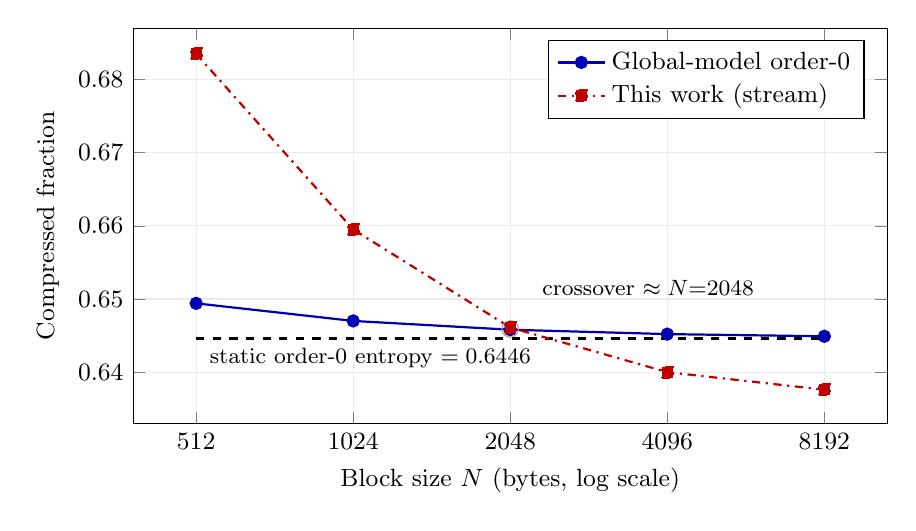
\begin{tikzpicture}
\begin{axis}[
  width=0.92\linewidth, height=6.6cm,
  xmode=log, log basis x=2,
  xtick={512,1024,2048,4096,8192},
  xticklabels={512,1024,2048,4096,8192},
  xlabel={Block size $N$ (bytes, log scale)},
  ylabel={Compressed fraction},
  ymin=0.633, ymax=0.687,
  ytick={0.64,0.65,0.66,0.67,0.68},
  legend pos=north east, legend cell align=left,
  grid=both, grid style={gray!16},
  tick label style={font=\small}, label style={font=\small},
  legend style={font=\small},
]
% static order-0 entropy floor (enwik9); data: experiments/scripts/global_model_baseline.py
\addplot[black, dashed, thick, forget plot] coordinates {(512,0.6446) (8192,0.6446)};
\node[anchor=north west, font=\footnotesize] at (axis cs:512,0.6446)
      {\,static order-$0$ entropy $=0.6446$};
\addplot[mark=*, thick, color=blue!70!black] coordinates {
 (512,0.6494)(1024,0.6470)(2048,0.6458)(4096,0.6452)(8192,0.6449)};
\addlegendentry{Global-model order-$0$}
\addplot[mark=square*, thick, dashdotted, color=red!75!black] coordinates {
 (512,0.6835)(1024,0.6595)(2048,0.6461)(4096,0.6400)(8192,0.6376)};
\addlegendentry{This work (stream)}
\draw[gray!70] (axis cs:2048,0.6459) circle (3pt);
\node[anchor=west, font=\footnotesize] at (axis cs:2260,0.6515)
      {crossover $\approx N{=}2048$};
\end{axis}
\end{tikzpicture}
\caption{Compressed fraction versus block size on \texttt{enwik9}: the idealised
globally-modelled order-$0$ baseline (one byte-frequency model shared over the whole
stream, each block independently framed) against our codec's stream mode. The two cross
near $N{=}2048$. The static global model is more compact at small blocks, where it avoids
the codec's $O(A\log N)$ per-block header; the block-adaptive codec wins at large blocks by
tracking the stream's non-stationarity, dropping below the corpus's static order-$0$
entropy ($0.6446$, dashed) that lower-bounds any single-model coder. Underlying fractions
(global-model order-$0$ / this work, stream) at $N=512,1024,2048,4096,8192$:
$0.6494/0.6835$, $0.6470/0.6595$, $0.6458/0.6461$, $0.6452/0.6400$, $0.6449/0.6376$.}
\label{fig:crossover}
\end{figure}

The price is throughput, and the picture is two-sided. Our compression falls from
$199$ to $35$\,MB/s, and decompression---which additionally searches during
unranking---from $38$ to $9$\,MB/s, as the block grows from $512$ to $8192$,
because the per-block ranking is super-linear in $N$. Kanzi's coders run the
other way: at small blocks their fixed per-block cost dominates, so at $N=1024$
all three streaming coders compress at only ${\approx}80$\,MB/s (ANS0; Huffman and
Range comparable), \emph{slower} than our $186$; but they scale
up with block size, and at the auto block where they reach their best ratio they
run near $1$\,GB/s---one to two orders of magnitude faster than our method at the
matching ratio. The streaming coders' speed advantage is thus realised precisely
at the large blocks our method does not require for ratio. At the small blocks where its
ratio is best our compression happens to outrun Kanzi's---but only because Kanzi's per-block
setup cost makes \emph{its} order-$0$ coders slow there; against the fastest table-driven
entropy stages (an FSE/tANS implementation such as \texttt{zstd}'s) it would not, and our
decoding stays slower at every block (Table~\ref{tab:enwik9}). We therefore make no
throughput claim: the method's standing rests on ratio and structure, not speed.
Section~\ref{sec:applications} identifies practical contexts in which the block
size is an external constraint and the small-$N$ ratio advantage becomes the
operative comparison.

Codecs that model context reach smaller fractions only by exploiting structure
our order-$0$ method does not, and are not order-$0$ baselines; for reference, at the auto
block the order-$1$ ANS1 reaches $0.4828$, FPAQ $0.5925$ and CM $0.4956$, and the
context-mixing TPAQ and TPAQX $0.1767$ and $0.1703$---the last below $8$\,MB/s.

\subsection{Heterogeneous corpora}\label{sec:silesia}
To test whether the small-block advantage on \texttt{enwik9} generalises beyond
text, we repeat the comparison on the Silesia corpus---twelve files of
deliberately mixed type (English and Polish text, program source, an executable, a
database, and medical images), $212$\,MB in total. Each file is compressed
independently at matched block sizes against Kanzi's Huffman coder, the most
compact streaming order-$0$ coder at small blocks (Table~\ref{tab:enwik9}).
Table~\ref{tab:silesia} gives the per-file fractions at $N=1024$.

\begin{table}[ht]
\centering
\renewcommand{\arraystretch}{1.15}
\caption{Per-file compressed fraction on the Silesia corpus at $N{=}1024$, each
file compressed independently, against Kanzi's Huffman coder (the most compact
streaming order-$0$ coder at this block). Lower is better; the smaller of each
pair is in bold. The method wins on every text and source file and loses only on
the dense, full-alphabet binaries; the aggregate is a tie.}
\begin{tabular}{l r c c}
\toprule
\textbf{File (type)} & \textbf{Size (MB)} & \textbf{This work} & \textbf{Huffman} \\
\midrule
\texttt{dickens} (text)       & $10.2$ & $\mathbf{0.6028}$ & $0.6106$ \\
\texttt{reymont} (text)       & $6.6$  & $\mathbf{0.6350}$ & $0.6392$ \\
\texttt{webster} (text)       & $41.5$ & $\mathbf{0.6595}$ & $0.6638$ \\
\texttt{xml} (markup)         & $5.3$  & $\mathbf{0.6482}$ & $0.6558$ \\
\texttt{samba} (source)       & $21.6$ & $\mathbf{0.6611}$ & $0.6703$ \\
\texttt{nci} (structured)     & $33.6$ & $\mathbf{0.3277}$ & $0.3309$ \\
\texttt{mozilla} (executable) & $51.2$ & $\mathbf{0.7079}$ & $0.7116$ \\
\texttt{sao} (binary)         & $7.3$  & $\mathbf{1.0342}$ & $1.0360$ \\
\texttt{mr} (medical)         & $10.0$ & $0.5210$ & $\mathbf{0.4890}$ \\
\texttt{ooffice} (library)    & $6.2$  & $0.8388$ & $\mathbf{0.8263}$ \\
\texttt{osdb} (database)      & $10.1$ & $0.9142$ & $\mathbf{0.9015}$ \\
\texttt{x-ray} (image)        & $8.5$  & $0.8857$ & $\mathbf{0.8376}$ \\
\midrule
Total                         & $211.9$ & $0.6477$ & $\mathbf{0.6473}$ \\
\bottomrule
\end{tabular}
\label{tab:silesia}
\end{table}

The outcome is a clean split along alphabet width. On every text and source
file---\texttt{dickens}, \texttt{reymont}, \texttt{webster}, \texttt{xml},
\texttt{samba}---and on the structured \texttt{nci}, our method is the more
compact; it loses only on the dense, full-alphabet binaries \texttt{mr},
\texttt{ooffice}, \texttt{osdb} and \texttt{x-ray}. This is exactly what
Proposition~\ref{prop:order0} predicts: the per-block housekeeping is
$O(A\log N)$, negligible when the alphabet $A$ is small but, on a near-$256$-symbol
source, large enough to overtake the gain from exact arrangement coding. The
prediction is quantitative---the deficit on the full-alphabet \texttt{x-ray} image
falls from $0.048$ at $N{=}1024$ to $0.014$ at $N{=}8192$ as the fixed header
amortises over a larger block---and the aggregate gap to Huffman is only
$+0.0004$, $+0.0028$, $+0.0022$, $+0.0004$ at $N{=}1024,2048,4096,8192$: a tie to
within $0.4\%$ on a corpus chosen to be hostile, with our method winning the
majority of files outright.

Two further points connect this to the rest of the section. First, the text files
independently reproduce the \texttt{enwik9} result---on narrow-alphabet data the
method beats Huffman---so that advantage is a property of the alphabet, not of a
single benchmark. Second, the per-file figures isolate the amortisation effect
noted above: compressed as one concatenated stream the corpus yields $0.6501$ at
$N{=}1024$ against $0.6477$ per file, the $0.0024$ difference being the cost of the
stream-global alphabet once the byte distribution shifts between files. The
practical reading is that this codec is the most compact of the \emph{block-resetting}
order-$0$ coders for constrained-alphabet inputs at small blocks, and is competitive
rather than preferable on wide-alphabet, heterogeneous data.

These per-file wins are over Huffman, which both the integer-length penalty and per-block
table resets handicap. Against the sterner globally-modelled order-$0$ baseline introduced
above (Figure~\ref{fig:crossover}), the picture refines along the same stationarity axis:
on the \emph{stationary} text files (\texttt{dickens}, \texttt{reymont}, \texttt{webster})
one global model is the better fit and edges our codec, whereas on the structured,
non-stationary files---\texttt{xml}, the source tree \texttt{samba}, the executable
\texttt{mozilla}---our per-block counts adapt to the shifting local statistics and our
codec is the more compact. The codec's ratio advantage over a strong order-$0$ baseline is
thus specific to non-stationary data; on stationary text it is the structural package, not
ratio, that sets it apart.

The classic Canterbury corpus ($2.8$\,MB, eleven mostly textual files, each at
$N{=}1024$) reproduces the pattern---the method wins nine of eleven files and the
aggregate ($0.4803$ against Huffman's $0.4806$), losing only the wide-alphabet
binaries---and the larger Canterbury files extend it, the four-symbol \texttt{E.\,coli}
genome showing the widest narrow-alphabet margin ($0.256$ against $0.279$). The most
telling single file is the bilevel fax image \texttt{ptt5}: narrow and highly skewed, it
reaches $0.150$ where Huffman manages $0.224$. That gap has a different cause from the
housekeeping differences seen elsewhere---Huffman must spend a whole bit on the dominant
symbol whatever its probability, whereas the exact rank pays only its true information
content---so on skewed sources the method's edge over Huffman is the avoidance of the
integer-length-code penalty an arithmetic coder also escapes, here realised by
combinatorial ranking.
\subsection{Stream versus per-record mode}\label{sec:modeexp}
Section~\ref{sec:modes} distinguishes a \emph{stream} mode, which amortises a
reference alphabet across the blocks, from a \emph{per-record} mode in which each
block names its own alphabet. Compressing the same input both ways isolates exactly
what that amortisation is worth. On \texttt{enwik9}---one homogeneous text
stream---stream mode is the more compact at every block size, and the margin grows
as the block shrinks and the per-block alphabet cost is paid more often
(Table~\ref{tab:modes}): from $0.3\%$ of the input at $N{=}8192$ to $1.5\%$ at
$N{=}512$. The stream column reproduces the ``this work'' fractions of
Table~\ref{tab:enwik9}, as it must, those experiments being stream mode.

\begin{table}[ht]
\centering
\caption{Stream versus per-record mode on \texttt{enwik9}: compressed fraction at
each block size. $\Delta$ is per-record minus stream---the alphabet amortisation
stream mode provides---and grows as the block shrinks, the per-block alphabet cost
then being paid more often.}
\begin{tabular}{r c c c}
\toprule
\textbf{$N$} & \textbf{stream} & \textbf{per-record} & $\Delta$ \\
\midrule
$512$  & $0.6835$ & $0.6938$ & $+0.0103$ \\
$1024$ & $0.6595$ & $0.6676$ & $+0.0082$ \\
$2048$ & $0.6461$ & $0.6528$ & $+0.0067$ \\
$4096$ & $0.6400$ & $0.6442$ & $+0.0042$ \\
$8192$ & $0.6376$ & $0.6397$ & $+0.0021$ \\
\bottomrule
\end{tabular}
\label{tab:modes}
\end{table}

The Silesia files, compressed one at a time, show that the better mode tracks
alphabet homogeneity rather than being universal. On the text and source files the
reference fits and stream mode wins, by up to $0.010$ at $N{=}512$
(\texttt{reymont}; similarly \texttt{dickens}, \texttt{webster}, \texttt{xml},
\texttt{samba}). On the dense, wide-alphabet binaries the per-block alphabet varies
so much that encoding each block's symmetric difference against a fixed reference
costs \emph{more} than naming its alphabet outright, and per-record mode is the more
compact---\texttt{mr} by $0.015$ ($2.9\%$) and \texttt{mozilla} by $0.006$ at
$N{=}512$, with \texttt{ooffice}, \texttt{sao}, and \texttt{x-ray} at best neutral.
These are the same wide-alphabet files on which the method trails Huffman
(Section~\ref{sec:silesia}): where the order-$0$ housekeeping is already
proportionally large, a mismatched reference only adds to it. The rule is the one
Section~\ref{sec:modes} states---stream mode for homogeneous record streams,
per-record for independent or alphabet-varying units---now with the cost of choosing
wrong made explicit.

\subsection{A record store}\label{sec:recordstore}
Section~\ref{sec:applications} argues that the method's home is the homogeneous
record store, so we test one on real data: the timestamp column of the \textsc{Hadoop}
log set from the loghub collection~\cite{loghub2023}---$180\,897$ records, the ISO-8601
field \texttt{YYYY-MM-DD HH:MM:SS,mmm} that opens each log line, $23$ bytes each over a
$14$-symbol alphabet---compressed at record granularity with the block equal to the
record. The defining property of a store is
that records are written, addressed, encrypted, and read \emph{individually}, so the
only admissible coders are those that preserve per-record access;
Table~\ref{tab:recordstore} compares them, with whole-stream \texttt{gzip} included
only as a ceiling.

\begin{table}[ht]
\centering
\caption{A record store of $180\,897$ real timestamp records from the loghub
\textsc{Hadoop} log set ($23$ bytes each, $14$-symbol alphabet), compressed at record
granularity (block $=$ record). Only coders preserving per-record access are candidates;
a static global-model order-$0$ coder is the most compact of them, but---unlike the
method---offers no in-place encryption, count-indexed queryability, or exact predictable
per-block size.}
\begin{tabular}{l c c}
\toprule
\textbf{Coder} & \textbf{Per-record access} & \textbf{Fraction} \\
\midrule
Global-model order-$0$            & yes & $0.5544$ \\
This work, stream mode          & yes & $0.8048$ \\
This work, per-record mode      & yes & $1.0689$ \\
\texttt{gzip\,-9}, per record   & yes & $1.8679$ \\
\texttt{gzip\,-9}, whole stream & no  & $0.1082$ \\
\bottomrule
\end{tabular}
\label{tab:recordstore}
\end{table}

Among the access-preserving coders the static global-model coder is the most compact
($0.554$): coding each record against one stream-wide frequency table, it pays no
per-record model cost. Our stream mode ($0.805$) trails it---it re-derives an alphabet
symmetric difference and per-symbol counts for every record---while per-record mode
($1.069$, the full alphabet on each $23$-byte record) and per-record \texttt{gzip}
($1.868$, a multi-byte header each) expand outright. On ratio alone, then, the codec is
not the coder of choice here: a global model wins, and---to be fair to the strongest
alternative---that global model can itself be encrypted record by record with AES-CTR,
matching our full mode on size, per-record access, and length-only leakage. Two things that
pairing still does not provide are an exact per-block size known \emph{before} encoding
(fixed by $(N,k)$ in our representation, useful for fixed-rate channels and buffer
budgeting) and the count-indexed \emph{queryable} dial of Section~\ref{sec:encryption},
which lets a key-less party compute over the ciphertext at no size cost. Those two
properties, not ratio and not encryption \emph{per se}, are the reason to choose the method
in this setting. Whole-stream \texttt{gzip} reaches $0.108$, far below
all of them, because the timestamps span a short window and recur heavily (only $64\%$ are
distinct) and \texttt{gzip} exploits that inter-record redundancy; but it forfeits
per-record access entirely---it cannot decompress, re-encrypt, or address one record
without processing the rest---so it is a ceiling, not a substitute. On
record stores whose records are larger or whose alphabets are constrained---short-read
genomics being the worked example of Section~\ref{sec:genomics}---the method is
additionally competitive on ratio.

\subsection{Effect of alphabet size}
Because the method is order-$0$, its compressed fraction on an input drawn
uniformly from an alphabet of $A$ symbols should approach the order-$0$ entropy
$\tfrac{1}{8}\log_2 A$. To verify this, we generated $64$\,MiB of uniform random
bytes restricted to $A$ distinct values for several $A$ and compressed each at two
block sizes, alongside Kanzi's Huffman coder at its default auto block
(Table~\ref{tab:alphabet}).

\begin{table}[ht]
\centering
\renewcommand{\arraystretch}{1.15}
\caption{The method on uniform random bytes over an $A$-symbol alphabet, at two block sizes,
alongside Kanzi's Huffman coder at its auto block ($64$\,MiB for the compressed fraction,
$256$\,MiB for throughput, the latter excluding our one-time cache build). The $N{=}1024$
and $N{=}4096$ columns are this work. The compressed fraction tracks the order-$0$ entropy
$\tfrac18\log_2 A$---within $0.001$--$0.010$ of Huffman at $N{=}4096$, the gap largest at
$A{=}256$ where per-block housekeeping is proportionally most significant---while throughput
runs $5$--$30\times$ below Huffman, the more so as the block grows.}
\begin{tabular}{r c c c c c c c}
\toprule
 & & \multicolumn{3}{c}{\textbf{Compressed fraction}} & \multicolumn{3}{c}{\textbf{Throughput (MB/s)}} \\
\cmidrule(lr){3-5}\cmidrule(lr){6-8}
\textbf{$A$} & $\tfrac{1}{8}\log_2 A$ & \textbf{$N{=}1024$} & \textbf{$N{=}4096$} & \textbf{Huff.} & \textbf{$N{=}1024$} & \textbf{$N{=}4096$} & \textbf{Huff.} \\
\midrule
$2$   & $0.1250$ & $0.1315$ & $0.1267$ & $0.1256$ & $244$ & $78$  & $1695$ \\
$4$   & $0.2500$ & $0.2573$ & $0.2519$ & $0.2506$ & $179$ & $48$  & $1497$ \\
$16$  & $0.5000$ & $0.5107$ & $0.5032$ & $0.5010$ & $185$ & $57$  & $924$  \\
$64$  & $0.7500$ & $0.7675$ & $0.7564$ & $0.7518$ & $173$ & $105$ & $1580$ \\
$256$ & $1.0000$ & $1.0537$ & $1.0131$ & $1.0028$ & $135$ & $132$ & $1225$ \\
\bottomrule
\end{tabular}
\label{tab:alphabet}
\end{table}

The fraction tracks $\tfrac18\log_2 A$ across the range, confirming order-$0$ optimality
on controlled inputs; at $N{=}4096$ it sits within $0.001$--$0.010$ of Huffman, the residual
being per-block housekeeping that shrinks as the block grows or the alphabet narrows. Two
points carry to the rest of the paper: compression improves as the alphabet narrows---a
four-symbol source compresses to the two-bit limit $0.25$, while a full-byte uniform source
is incompressible at order $0$ and both coders expand slightly---and the housekeeping is
proportionally largest exactly when the payload is smallest (small blocks, wide alphabets).
The right-hand columns expose the throughput cost: the method runs $5$--$30\times$ below
Huffman, and its speed tracks the magnitude of the ranks rather than the alphabet
alone---a narrow alphabet is quickest at a small block yet slowest at a large one, where
each rank approaches the central binomial coefficient and big-integer arithmetic dominates.

\subsection{Real constrained-alphabet data}\label{sec:genomics}
The synthetic sweep above draws bytes uniformly over an $A$-symbol alphabet; real
constrained-alphabet data lets us confirm the same behaviour outside the
laboratory and separates two regimes the method treats very differently. We
extract the nucleotide stream---the bases only, with quality scores and headers
excluded---from short-read sequencing data and compress it as an
$\{$A,C,G,T$\}$ byte stream at the read granularity.

On \emph{Escherichia coli} K-12 (accession \texttt{SRR2627175}, Illumina MiSeq)
the base composition is almost perfectly uniform: the four bases occur with
frequencies $0.244$--$0.256$ and the empirical order-$0$ entropy is $1.9999$
bits/base, an ideal fraction of $0.2500$. At $N{=}1024$ the method compresses the
$540$\,MB base stream to $0.2569$---reproducing, on real data, the synthetic
$A{=}4$ figure of $0.2573$ (Table~\ref{tab:alphabet}) to three decimals, a
direct confirmation that the alphabet model of Proposition~\ref{prop:order0}
describes real sequences. But a uniform four-symbol source is exactly the case in
which the order-$0$ floor coincides with trivial two-bit packing: the method
\emph{matches} the floor and, at small blocks, pays a slight housekeeping premium
over packing ($0.2569$ against $0.2500$). On near-uniform genomes it therefore has
no ratio advantage over bit-packing---only exactness and the structural properties
of Section~\ref{sec:applications}. (The assembled genome of the same organism
appears as a static file in the Canterbury corpus of Section~\ref{sec:silesia},
where its identically near-uniform composition again leaves the method just above
the two-bit floor.)

The advantage appears when the base composition is skewed. The genome of
\emph{Plasmodium falciparum} is among the most AT-rich known
(${\approx}80\%$ A$+$T genome-wide), and even after the GC-enrichment of
short-read sequencing its reads remain markedly non-uniform. On an Illumina run of
this organism (accession \texttt{ERR006177}) the base stream has frequencies
$A{=}0.327$, $T{=}0.359$, $C{=}0.162$, $G{=}0.153$ and an order-$0$ entropy of
$1.897$ bits/base---an ideal fraction of $0.237$, well below the two-bit ceiling.
At $N{=}1024$ the method compresses the $279$\,MB base stream to $0.2436$, against
$0.25$ for a two-bit pack: here exact arrangement coding is strictly the more
compact, because the single-symbol skew it captures is precisely what fixed-width
packing cannot. The residual $0.007$ over the $0.237$ floor is the same per-block
housekeeping seen throughout, and shrinks as the block grows. The comparison drawn
here is against fixed-width packing and \texttt{gzip}, not against the global-model
order-$0$ baseline of Figure~\ref{fig:crossover}: a single base-frequency model shared
over the stream would capture the same single-symbol skew and reach a comparable fraction,
so on this near-stationary source the method's case is again the structural package
(exact read sizing, in-place encryption) rather than a ratio win over a global model.

Two caveats temper this. First, the gains live in the base composition alone:
the order-$0$ model captures single-symbol skew, not the repeats and context that
dominate genomic redundancy. On this shuffled stream of short reads a general
LZ-plus-Huffman coder finds little such structure---\texttt{gzip\,-9} reaches only
$0.252$, which the exact ranking in fact edges---but reference-based, format-aware
genomic compressors such as CRAM and Genozip exploit alignment and context to
compress sequencing data far further, and remain the right choice in practice.
Second, quality scores and headers, the bulk of a FASTQ file, are a different
distribution we do not address. The genomics result is thus a validation of the
constrained-alphabet behaviour and an illustration of where exact order-$0$ coding
beats both bit-packing and an order-$0$-grade general compressor, not a claim to
competitive sequence compression.

These results position the present method as a simple, exactly invertible
order-$0$ coder that provably meets the order-$0$ entropy bound, rather than as a
competitor to context-modelling entropy coders. Its distinguishing properties lie
elsewhere: the encoding is a pure combinatorial rank, every block is
independent---enabling the straightforward parallelism of
Section~\ref{sec:implementation}---and the same machinery lends itself to
encryption.

\subsection{Encryption overhead}\label{sec:encexp}
The size-preserving cipher of Section~\ref{sec:encryption} adds no bytes: in every
setting the encrypted block is bit-for-bit the same size as the plaintext block, a
property our round-trip tests verify exactly. Its only cost is throughput, which
Table~\ref{tab:encryption} measures on a representative mildly skewed block over a
$40$-symbol alphabet (Apple~M3), comparing the plaintext codec against the two cipher
settings: \emph{queryable} (only the alphabet rank and the position ranks encrypted,
the counts left in clear) and \emph{full} (every field encrypted).

\begin{table}[ht]
\centering
\renewcommand{\arraystretch}{1.15}
\caption{Throughput cost of the size-preserving cipher on a representative block
(Apple~M3), plaintext versus the queryable and full settings. The compressed size is
identical in all three---the cipher adds exactly $0$ bytes. Throughput is in MB/s;
the parenthesised factor is the slowdown relative to plaintext. The plaintext figures
are not comparable with Table~\ref{tab:enwik9}: this is a different, deliberately small
representative block (a $40$-symbol alphabet at the sizes shown), chosen to isolate the
cipher's relative cost rather than absolute codec speed. The keystream is a
reference \texttt{SHA-256} construction, so these figures are an upper bound on the
overhead.}
\begin{tabular}{r l c c c}
\toprule
\textbf{$N$} & \textbf{Operation} & \textbf{Plaintext} & \textbf{Queryable} & \textbf{Full} \\
\midrule
$1024$ & compress   & $68.7$ & $38.3$ ($1.8\times$) & $31.7$ ($2.2\times$) \\
$1024$ & decompress & $11.1$ & $9.7$ ($1.1\times$)  & $9.3$ ($1.2\times$)  \\
$4096$ & compress   & $50.8$ & $40.6$ ($1.3\times$) & $38.6$ ($1.3\times$) \\
$4096$ & decompress & $10.0$ & $9.4$ ($1.1\times$)  & $9.2$ ($1.1\times$)  \\
\bottomrule
\end{tabular}
\label{tab:encryption}
\end{table}

Three things stand out, all consistent with the construction. First and most
important, encryption is \emph{exactly} size-preserving: every field is replaced by a
ciphertext over the same modulus, so the block length is unchanged and the only
information an encrypted store leaks is that length
(Section~\ref{sec:dial}). At the whole-file level the encrypted format adds a single
fixed-size header---a one-byte mode flag and a $16$-byte random salt---independent of
the input size and of the block count, so the per-block size cost remains exactly
zero. Second, the overhead falls almost entirely on
\emph{compression at small blocks}, where the plaintext codec is fastest and the
per-field keystream is therefore proportionally most expensive: up to $2.2\times$ for
full mode at $N{=}1024$. Decompression, already dominated by the downward search of
the unranking step---which the cipher never touches---absorbs the keystream cost
almost entirely, slowing by at most $1.2\times$. Third, full mode costs only modestly
more than queryable: the bulk of the work is encrypting the variable-width ranks,
which both settings share, while full mode adds one short keystream per count. As the
block grows the relative overhead shrinks, the per-field cost amortising over more
bytes.

Two qualifications apply. The keystream is a reference \texttt{SHA-256}
counter construction, chosen for clarity rather than speed, generated and reduced
per field behind a fresh big-integer allocation each time. Measured directly, that
reference generator runs at a flat ${\approx}0.7$\,GB/s irrespective of output size,
whereas a hardware-accelerated AES stream reaches an order of magnitude more---but
only once the output is large enough to amortise the cipher's per-call key schedule.
At the small per-field sizes this implementation requests, that setup cost dominates
and the cipher family barely matters; the order-of-magnitude gain is unlocked only by
generating one keystream per block and slicing the fields from it. The table is
therefore a deliberate \emph{upper bound}, not the operative cost: the headline
$2.2\times$ reflects the reference \texttt{SHA-256} per-field generator, and a per-block
keystream paired with a vetted cipher (AES where hardware support exists, ChaCha20 as the
portable alternative) would cut it substantially. The reader should read these figures as
the worst case the construction admits rather than its intended cost.
The figures are also for the cipher in isolation: a production
encrypted store would add per-block authentication (Section~\ref{sec:encryption}),
whose cost is not included here.

It is worth being precise about what the construction does and does not buy over a
conventional cipher. The obvious alternative is to compress, then encrypt with a stream
cipher such as AES-CTR, which is itself size-preserving. Two variants matter
(Table~\ref{tab:aesctr}). Encrypting the \emph{whole} compressed stream makes every record
opaque \emph{and} unaddressable---the record boundaries vanish into the ciphertext---so it
is no use to a store. Encrypting \emph{each record} independently, however (nonce $=$ record
index, the length framing left in clear), is size-preserving, per-record addressable, and
leaks only the per-record length---matching our \emph{full}-encryption mode on every axis,
and doing so more simply and faster, since it avoids the per-field big-integer keystream
whose cost Table~\ref{tab:encryption} reports. Full mode is therefore best understood as a
\emph{structurally integrated} alternative to per-record AES-CTR---encryption folded into
the coding pass, matching it on size, access, and leakage---not a more capable one; the
queryable mode below is where the construction does something no whole-record cipher can.

What no whole-record cipher can do is our \emph{queryable} mode. Leaving the per-record
counts in clear turns their cleartext field widths into a skip-table, so a key-less storage
server can read each record's count spectrum and field offsets and act on them---repack and
defragment the store, tier records by their (leaked) order-$0$ size, or pre-filter before an
authenticated equality check---without decrypting a byte or learning a symbol label. That
bounded, key-less computability at zero size cost is the construction's distinctive
offering, and it is exactly the deliberate trade of Section~\ref{sec:dial}: justified only
where such a query is wanted and the count-spectrum disclosure (Naveed--Kamara--Wright)
is acceptable, not as a default.

\begin{table}[ht]
\centering
\caption{The joint cipher versus stream-cipher alternatives. All four are exactly
size-preserving ($1.00\times$); they differ only in what a key-less party can compute.
Per-record AES-CTR matches full mode on every axis---size, per-record access, and
length-only leakage---and is simpler and faster; only the queryable dial exposes the count
spectrum and field offsets to a key-less party, which no whole-record cipher provides.
Whole-stream AES-CTR additionally forfeits per-record addressability.}
\renewcommand{\arraystretch}{1.15}
\begin{tabular}{l l}
\toprule
\textbf{Encrypted form} & \textbf{Computable without the key} \\
\midrule
Joint cipher, full mode       & per-block length only \\
Per-record AES-CTR            & per-block length only \\
Joint cipher, queryable mode  & count spectrum $+$ field offsets \\
Whole-stream AES-CTR          & nothing (records not addressable) \\
\bottomrule
\end{tabular}
\label{tab:aesctr}
\end{table}

\section{Applications}\label{sec:applications}
The codec's throughput is lower than streaming entropy coders at the same ratio,
so its value lies not in general-purpose compression but in a setting the
combinatorial representation suits unusually well: \emph{homogeneous record
stores}---collections of small, like-formatted records (database columns, log and
packet stores, sequencing reads) compressed and accessed one record at a time. Such
records share an alphabet, so the stream-mode reference of
Section~\ref{sec:modes} is fair; the block is the record, so the small-block regime
is the operative one rather than a contrivance; and, because each block is encoded as
integer fields over known finite ranges, the representation delivers as one package what a
streaming coder cannot: order-$0$-compact ratios, independent and parallel coding,
random access to any record, exact predictable size, and the size-preserving
cipher with count-indexed queryability of Section~\ref{sec:encryption}. The subsections below
develop this use case and the structural properties it draws on.

\subsection{Compressed record stores}
Here the small-block regime is not a contrivance but the only admissible one---the block
\emph{is} the externally fixed record---and it is exactly where this method is the most
compact of the \emph{block-resetting} order-$0$ coders on narrow-alphabet inputs
(Section~\ref{sec:computational-experiments}). Section~\ref{sec:recordstore} measures this on
$180\,897$ real log timestamps, where a static global model wins on ratio but only the
method supplies the encryption, queryability, and exact sizing a store needs.

Short-read sequencing is a second setting the experiments reach directly. Platforms
produce reads of roughly 50--300 bases, each a natural compression unit---fixed-length,
small, and over a four-symbol alphabet for which the method provably reaches the
order-$0$ floor in one pass with no model state. On real reads
(Section~\ref{sec:genomics}) it tracks that floor and, on the AT-rich
\emph{P.\ falciparum}, beats both fixed-width packing and \texttt{gzip} on the base
stream; dedicated formats such as CRAM still win overall through higher-order modelling,
but for an embedded sequencer or streaming edge device a simple, exactly invertible
coder at the read granularity may be preferable to a complex pipeline.

Other naturally small-record settings fit the same profile, though we report them as
motivated rather than measured: embedded and latency-bounded pipelines, where a large
amortising block simply will not fit; and packet or log stores---DNS responses, CAN
frames, fixed-width database rows---where the record is the only available granularity
and the per-block housekeeping is proportionally smallest relative to the payload.

One caveat applies across all these settings: the decoder is markedly slower than the
encoder---roughly four to five times so (Table~\ref{tab:enwik9}), owing to the downward
search in the unranking step---so read-heavy deployments such as record stores and
sequencing archives, written once and read many times, must weigh that asymmetry against
the ratio gain; accelerating the unranking search
(Section~\ref{sec:decompression-algorithm}) is the natural remedy.

\subsection{Further structural uses}
Beyond storage, the exactness has uses of its own. A block's compressed size is fixed by
$(N,k)$ and known before encoding---convenient for fixed-rate channels and buffer
budgeting---and the coding is exact integer arithmetic with no renormalisation, a clean
reference against which to validate faster, approximate coders; the underlying $O(k)$
rank/unrank bijection is independently useful for compact set identifiers and sampling.
And because encoding an occurrence bitset as its colexicographic rank is exactly the
construction underlying succinct rank/select bitvectors, the codec doubles as a building
block for compressed-but-queryable structures---bitmaps, inverted-index posting lists, and
similar set- or permutation-structured data, for which an order-$0$ model is already
near-optimal.
\section{Discussion}\label{sec:discussion}
The experiments and the construction together place the method precisely, and it
is worth being explicit about where that is, and is not.

Proposition~\ref{prop:order0} and the experiments agree that the codec attains the
order-$0$ entropy of its input: its arrangement coding is exact, free of the
integer-length penalty that costs Huffman on skewed sources---the \texttt{ptt5}
case of Section~\ref{sec:silesia}---and of the renormalisation state a streaming
coder carries. What it cannot do is model structure above order~$0$. On data whose
redundancy is largely higher-order---natural text beyond its symbol frequencies,
genomic reads with repeats---context-modelling and dictionary coders (the
CM/TPAQ family, CRAM, Genozip, or simply \texttt{gzip} exploiting matches) compress
substantially further and remain the right tools when ratio is the only concern.
The method's compression claim is a claim about the order-$0$ frontier, not the
absolute one.

Within that frontier the codec is the most compact of the \emph{block-resetting} order-$0$
coders on narrow-alphabet inputs at matched block sizes, and \texttt{ptt5}
(Section~\ref{sec:silesia}) shows that edge can be large where a skewed distribution defeats
Huffman's integer-length codes. Three bounds, established with the data in
Section~\ref{sec:computational-experiments} and not re-argued here, keep that edge in
proportion: on a heterogeneous corpus it is a fraction of a percent and reverses on
wide-alphabet binaries as the $O(A\log N)$ housekeeping predicts; part of it is stream
mode's alphabet amortisation rather than the coding kernel; and against a coder granted one
global model it reverses outright below the crossover (Figure~\ref{fig:crossover}). Ratio
alone is therefore not the reason to choose the method. The reason is structural: because
each block is a tuple of finite-range integers rather than a self-delimiting bitstream, one
representation packages independent, randomly-accessible blocks---which block-resetting
coders also allow---with two things a self-delimiting bitstream does not give: an exact size
known before encoding, and the size-preserving, queryable cipher of
Section~\ref{sec:encryption}. That package, paired with order-$0$
compactness, is why the method's home is the homogeneous record store, shown here on real
production-log timestamps and genomic reads.

The price is throughput. Big-integer arithmetic makes the codec slower than
table-driven coders at the same ratio, and decoding---which additionally searches
during unranking---is several times slower than encoding, a real consideration for
read-heavy stores. The encryption, finally, is offered with a security argument
rather than a formal proof: it reduces the scheme's confidentiality to that of a
standard keystream and states its residual leaks (the per-field modulus and the
per-block length), but any deployment needs a vetted stream cipher, disciplined
nonces, and review by a cryptographer. A hardened, formally analysed realisation is
the most valuable next step.

\section{Conclusions and future research}\label{sec:conclusions}
We have studied the representation that order-$0$ enumerative coding induces, realised as a
lossless byte-stream codec. Each fixed-length block is decomposed into one bitset per byte
value; after a length-reduction step the bitsets are replaced by their colexicographic
ranks, so that a block is a short tuple of integer fields---the per-symbol counts and these
ranks---each over a known finite range, and it is this finite-range structure, rather than
the codec as such, that carries the contribution. The experiments of
Section~\ref{sec:computational-experiments} confirm that the scheme is
order-$0$-optimal: on \texttt{enwik9} its compressed size converges, as the
block grows, onto the order-$0$ rate the Huffman, range, and ANS
entropy coders attain---and at a matched block size its stream mode is the more compact of
these \emph{block-resetting} coders---while on controlled inputs it tracks
$\tfrac18\log_2 A$ across alphabet sizes $A$. On the heterogeneous Silesia corpus that
small-block edge holds on every text and source file but reverses on the dense,
full-alphabet binaries as the $O(A\log N)$ housekeeping overtakes the gain---a tie in
aggregate---and against a coder granted one global model it reverses below the crossover;
ratio is therefore not the method's case, which rests instead on the structural package
(Section~\ref{sec:discussion}).

The method is consequently most effective on constrained byte universes: a
nucleotide source over $\{$A,C,G,T$\}$ compresses to its two-bits-per-symbol
limit, whereas a full-byte uniform source is incompressible at order $0$ and the
per-block overhead causes slight expansion. Its cost is throughput---the big-integer arithmetic makes it slower than
streaming entropy coders at the same ratio---so it is not a general-purpose
text compressor in the mould of \texttt{zstd} or \texttt{bzip2}. Its niche is
the complementary corner: architectures in which the block size is an external
constraint---embedded pipelines, packet and record stores, short-read
genomics---where small fixed blocks are the unit of storage and access and the
structural package, not ratio alone, is the operative advantage
(Section~\ref{sec:applications}). Beyond ratio, its
appeal follows directly from the combinatorial representation: blocks are
coded independently, which we exploit for a parallel pipeline, and each field of a
block is an integer over a known finite range, which admits a size-preserving cipher
that combines compression and encryption at no size cost.

Several directions remain. The dominant decompression cost is the downward search
in the unranking step, whose acceleration is worth pursuing~\cite{rulevskiy2022};
the hockey-stick identity for contiguous runs reduces big-integer additions and
may repay its detection cost on large blocks. A native or GMP-backed port is
unlikely to help substantially, since the bottleneck is large-integer addition,
which performs comparably under Go's \texttt{math/big} and GMP. More promising are
the structural avenues: a queryable, succinct variant that supports rank and
select on the compressed form without full decompression, and a hardened,
production realisation of the joint compression-encryption scheme of
Section~\ref{sec:encryption}---with a vetted stream cipher and a full security
analysis under a stated threat model. A dedicated hardware implementation is a further
natural direction: each rank is a multi-operand wide-integer sum that maps onto a
carry-save adder tree, the datapath needs only addition, comparison, and table lookup
(the coefficients being precomputed), and the independence of blocks gives spatial
parallelism, so an FPGA prototype would be a sensible first step.

% --- MDPI back matter (mandatory sections) ---
\authorcontributions{Conceptualization, methodology, software, validation, formal
analysis, investigation, writing---original draft preparation, and writing---review
and editing were all carried out by A.J.R., the sole author. The author has read and
agreed to the published version of the manuscript.}

\funding{This research received no external funding; the work was wholly self-funded.}

\dataavailability{The corpora used in this study are publicly available:
\texttt{enwik9}, the Silesia and Canterbury corpora, the loghub \textsc{Hadoop} log
dataset~\cite{loghub2023}, and the sequencing runs \texttt{SRR2627175}
(\emph{E.\ coli}) and \texttt{ERR006177} (\emph{P.\ falciparum}) from the ENA. The
reference codec, the experiment scripts that reproduce every table, and the sources that
generate this manuscript are openly available in a public repository (repository URL and
archival DOI to be inserted before submission).}

\acknowledgments{During the preparation of this manuscript the author used Claude
(Anthropic) to assist with drafting and editing the text and with surveying related
work; its use in the computational experiments is described in
Section~\ref{sec:computational-experiments}. The core method---the combinadic
compression algorithm and its codec---was conceived and developed independently and
solely by the author, predating this assistance. The author reviewed and verified all
AI-assisted output and takes full responsibility for the content of this publication.}

\conflictsofinterest{The author declares no conflicts of interest.}

\abbreviations{Abbreviations}{
The following abbreviations are used in this manuscript:
\\

\noindent
\begin{tabular}{@{}ll}
AES & Advanced Encryption Standard\\
ANS & Asymmetric numeral systems\\
CTR & Counter mode (block-cipher mode of operation)\\
ENA & European Nucleotide Archive\\
FPE & Format-preserving encryption\\
FPGA & Field-programmable gate array\\
GMP & GNU Multiple Precision Arithmetic Library\\
IND-CPA & Indistinguishability under chosen-plaintext attack\\
PRG & Pseudorandom generator\\
SHA & Secure Hash Algorithm
\end{tabular}
}

\reftitle{References}
\externalbibliography{yes}
\bibliography{article}

\PublishersNote{}

\end{document}
